\documentclass{standalone}
\usepackage{tikz}
\usepackage{verbatim}
\begin{document}
\pagestyle{empty}
  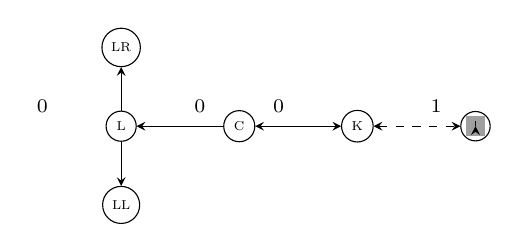
\begin{tikzpicture}
    \node[draw,circle,scale=2/3] (left_right) at (-1.5, 1) {\scriptsize LR};
    \node[draw,circle,scale=2/3] (left_left) at (-1.5, -1) {\scriptsize LL};
    \node[draw,circle,scale=2/3] (left) at (-1.5, 0) {\scriptsize L};
    \node[draw,circle,scale=2/3] (c) at (+0, 0) {\scriptsize C};
    \node[draw,circle,scale=2/3] (d) at (+1.5, 0) {\scriptsize K};
    \node[draw,circle,scale=2/3] (e) at (+3, 0) {\scriptsize S};
    \node[draw,rectangle,fill,gray!75] (r) at (+3, 0) {};
    \draw[-stealth]  (c) -- (left);
    \draw[-stealth]  (left) -- (left_right);
    \draw[-stealth]  (left) -- (left_left);
    \draw[stealth-stealth] (c) -- (d);
    \draw[stealth-stealth, dashed] (d) -- (e);
    \draw[-stealth]  (e) -- (r);
    \foreach \x in {-0.5, ..., 0.5} {
      \node at (\x, 0.25) {\scriptsize 0};
    }
    \node at (2.5, 0.25) {\scriptsize 1};
    \node at (-2.5, 0.25) {\scriptsize 0};
  \end{tikzpicture}
\end{document}